
We present the PDF of the inputs of the dynamical simulation and the
output PDF of the outputs after applying the polarization prior in
addition to the default priors.
%make use of subplots from matplotlib in order to plot all the posteriors
\label{app: results}

%%%%%%%%%%%%% TASK --- 

\clearpage
\begin{figure*}
	\begin{minipage}{180mm}
	\begin{center}
	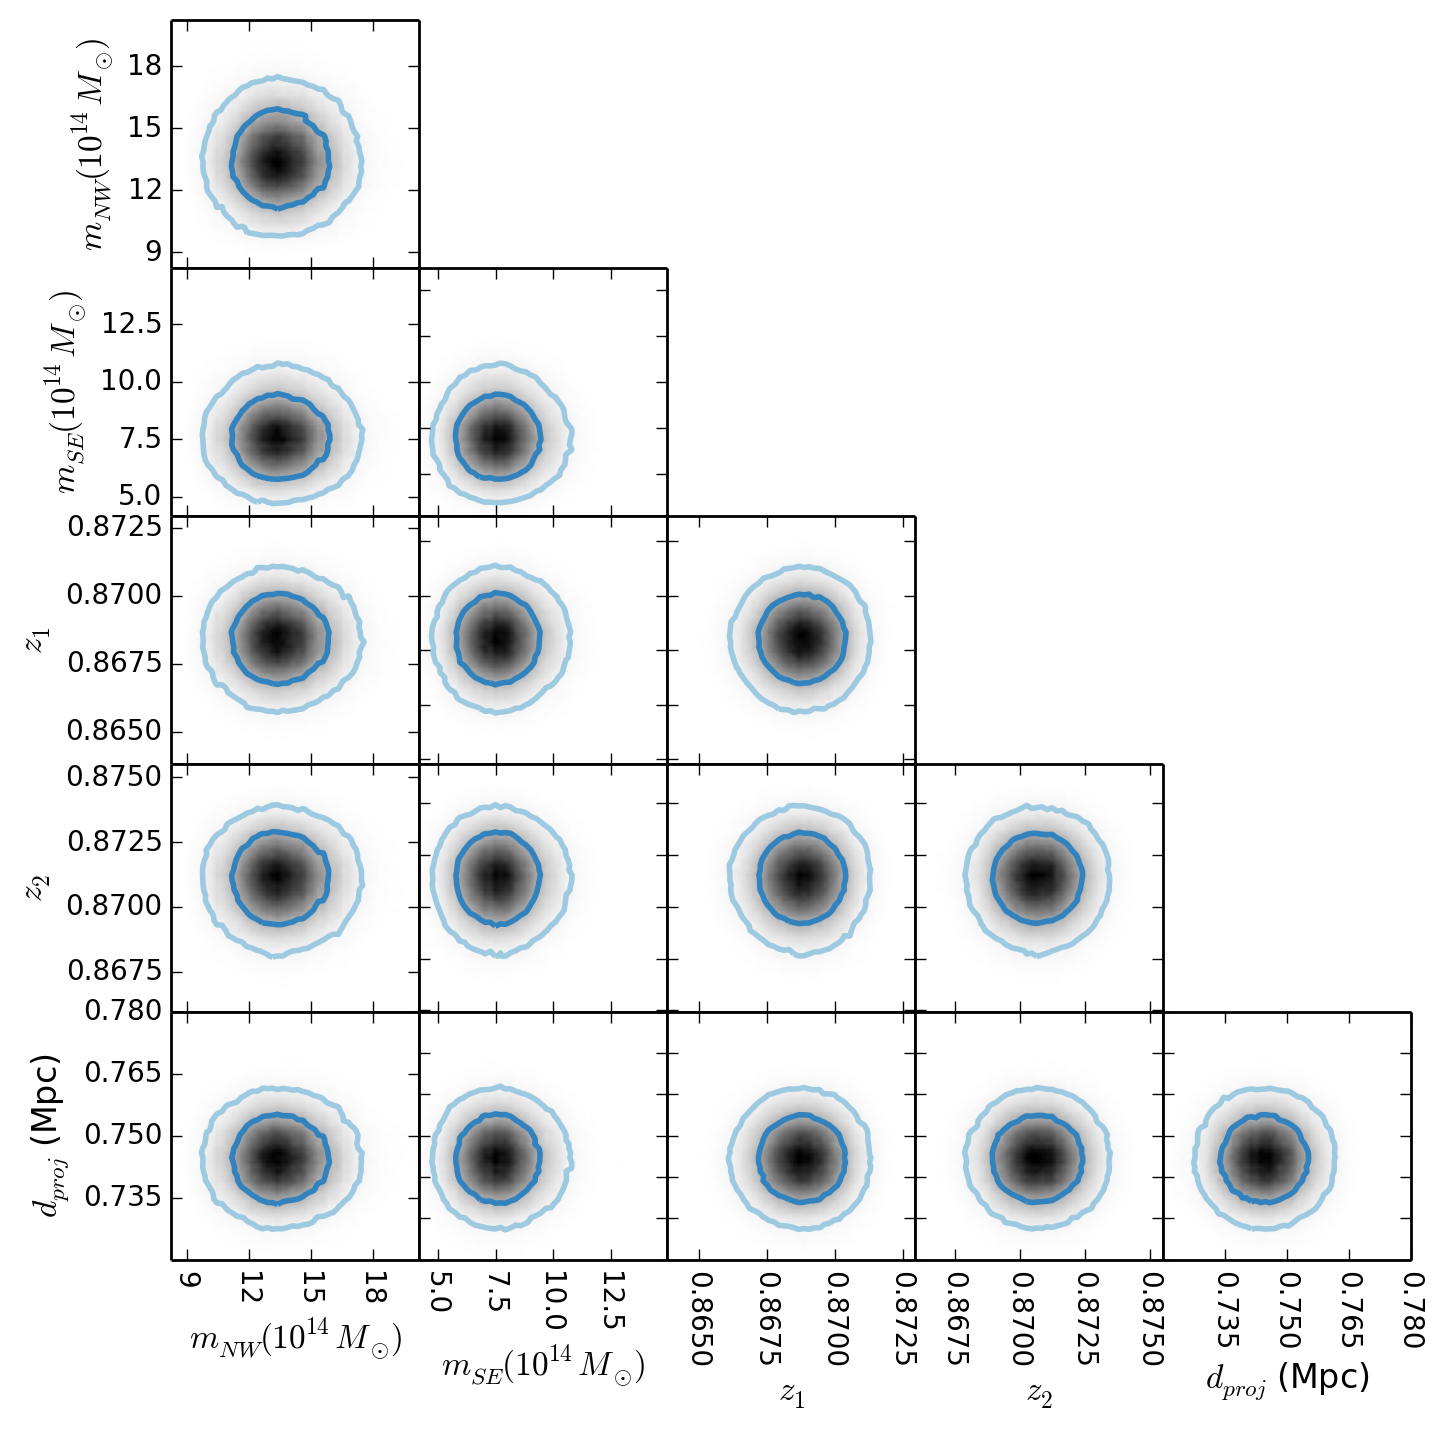
\includegraphics[width=0.7\linewidth]{TwoMnWBSG_inputsVsinput.png}
	\caption{The original inputs plotted against the inputs after
applying polarization prior and default priors. }
	\end{center}
	\end{minipage}
\end{figure*}

\begin{figure*}
\begin{minipage}{180mm}
	\begin{center}
	%\vspace{200px}
	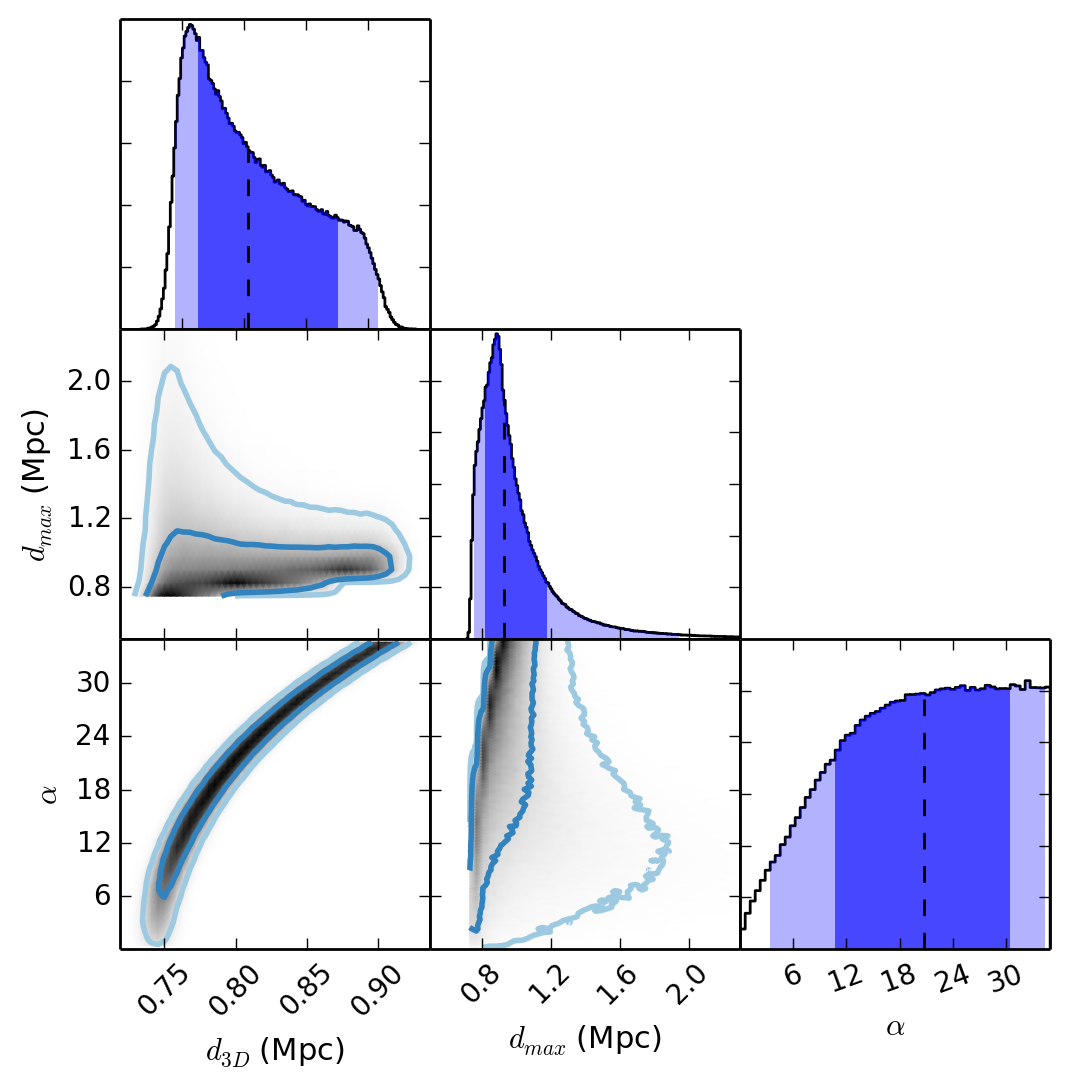
\includegraphics[width=0.5\linewidth]{TwoMnWBSG_tri_geo.png}
	\caption{Output PDF of characteristic timescales of the simulation
against the input PDF. }
	\end{center}
	\end{minipage}
\end{figure*}

\begin{figure*}
\begin{minipage}{180mm}
	\begin{center}
	%\vspace{200px}
	\includegraphics[width=0.7\linewidth]{TwoMnWBSG_geoVsinputs.png}
	\caption{Output PDF of characteristic timescales of the simulation
against the input PDF. }
	\end{center}
	\end{minipage}
\end{figure*}

\begin{figure*}
\begin{minipage}{180mm}
	\begin{center}
	%\vspace{200px}
	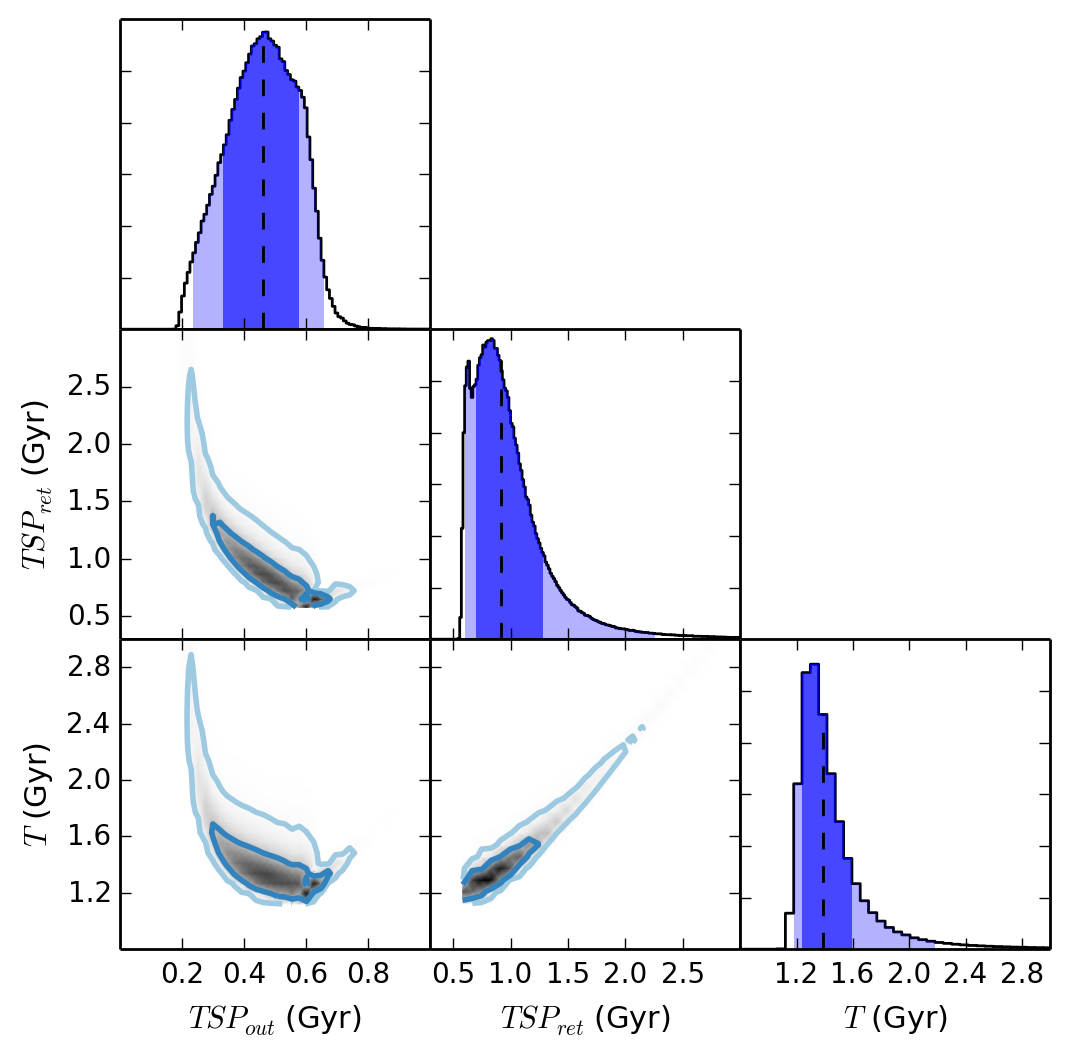
\includegraphics[width=0.5\linewidth]{TwoMnWBSG_tri_time.png}
	\caption{Output PDF of characteristic timescales of the simulation
against the input PDF. }
	\end{center}
\end{minipage}
\end{figure*}

\begin{figure*}
\begin{minipage}{180mm}
	\begin{center}
	%\vspace{200px}
	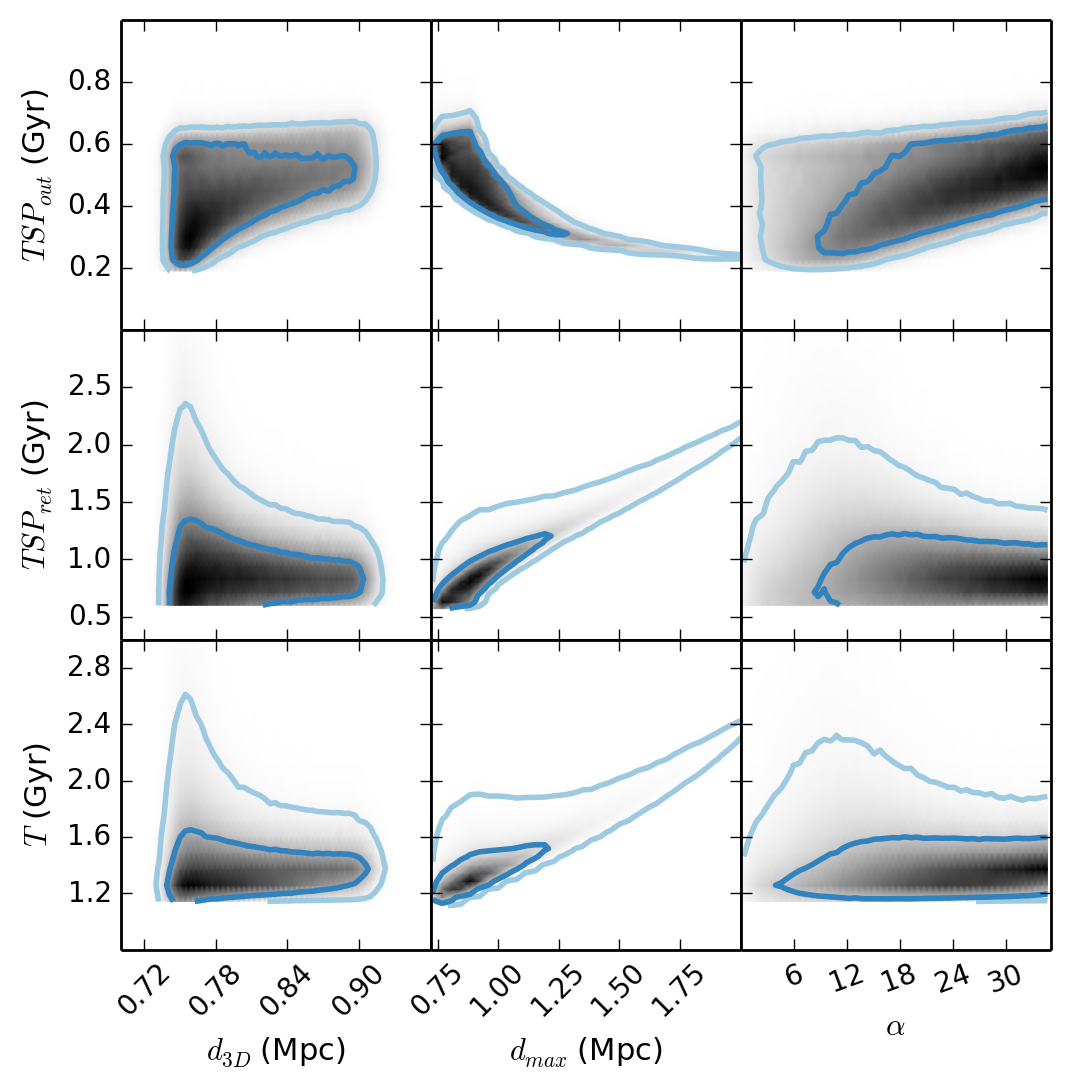
\includegraphics[width=0.5\linewidth]{TwoMnWBSG_timeVsgeo.png}
	\caption{Output PDF of characteristic timescales of the simulation
against the input PDF. }
	\end{center}
\end{minipage}

\end{figure*}
\begin{figure*}
\begin{minipage}{180mm}
	\begin{center}
	%\vspace{200px}
	\includegraphics[width=0.7\linewidth]{TwoMnWBSG_timeVsinput.png}
	\caption{Output PDF of characteristic timescales of the simulation
against the input PDF. }
	\end{center}
\end{minipage}
\end{figure*}


\begin{figure*}
\begin{minipage}{180mm}
	\begin{center}
	%\vspace{200px}
	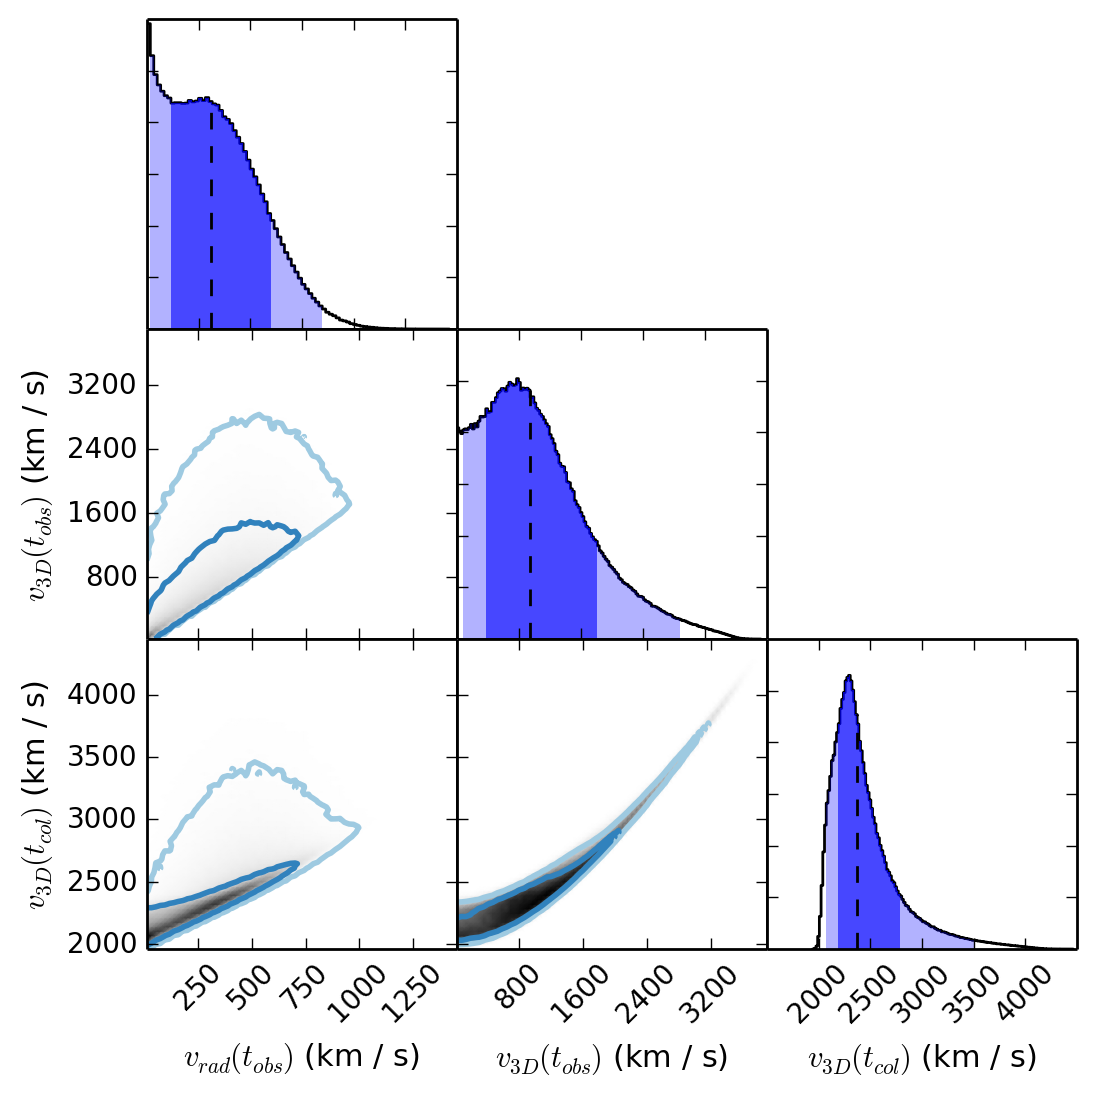
\includegraphics[width=0.5\linewidth]{TwoMnWBSG_tri_vel.png}
	\caption{Output PDF of characteristic timescales of the simulation
against the input PDF. }
	\end{center}
\end{minipage}
\end{figure*}

\begin{figure*}
\begin{minipage}{180mm}
	\begin{center}
	%\vspace{200px}
	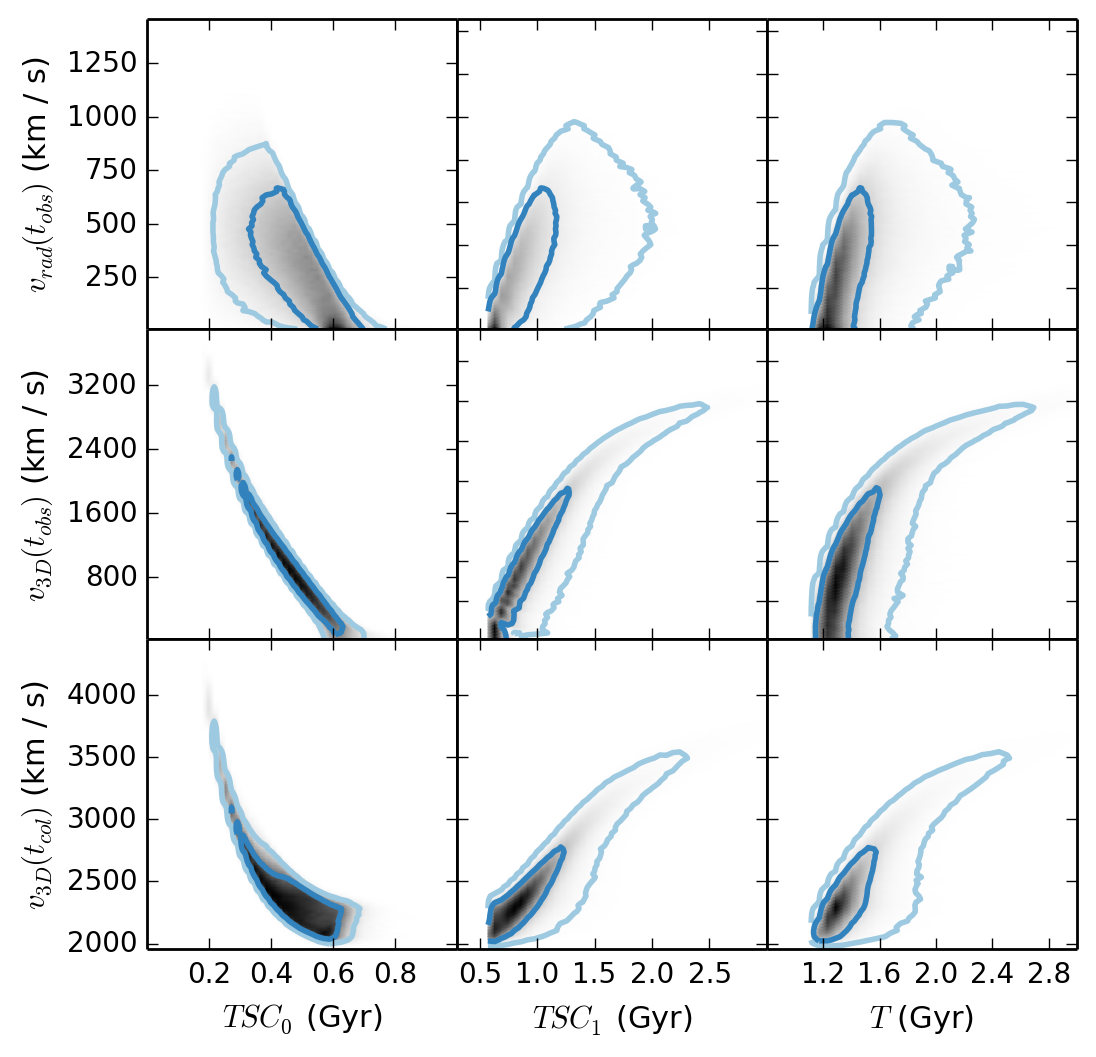
\includegraphics[width=0.5\linewidth]{TwoMnWBSG_velVStime.png}
	\caption{Output PDF of characteristic timescales of the simulation
against the input PDF. }
	\end{center}
\end{minipage}
\end{figure*}

\begin{figure*}
\begin{minipage}{180mm}
	\begin{center}
	%\vspace{200px}
	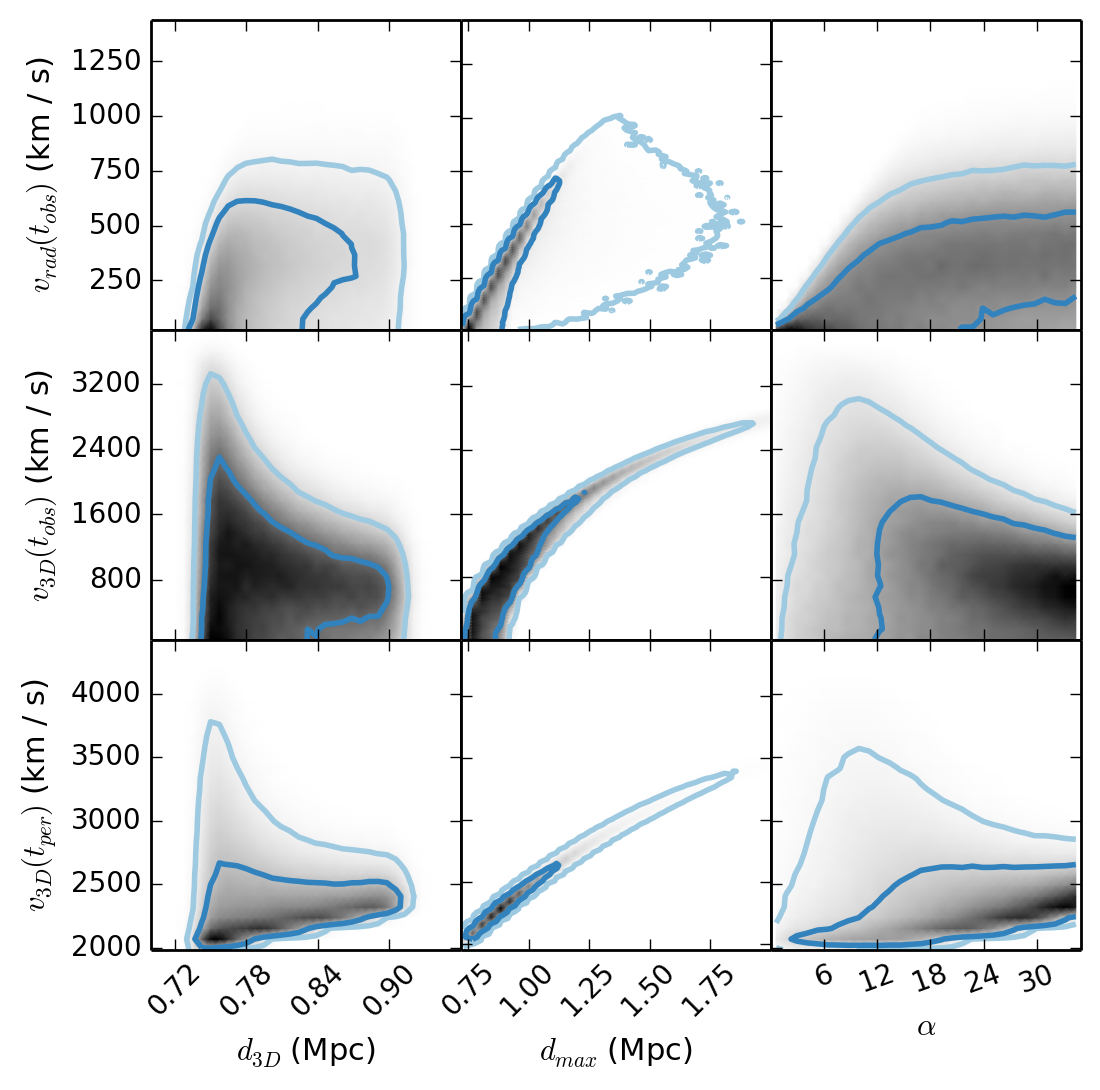
\includegraphics[width=0.5\linewidth]{TwoMnWBSG_velVSgeo.png}
	\caption{Output PDF of characteristic timescales of the simulation
against the input PDF. }
	\end{center}
\end{minipage}
\end{figure*}

\begin{figure*}
\begin{minipage}{180mm}
	\begin{center}
	%\vspace{200px}
	\includegraphics[width=0.7\linewidth]{TwoMnWBSG_velVsinputs.png}
	\caption{Output PDF of characteristic timescales of the simulation
against the input PDF. }
	\end{center}
\end{minipage}
\end{figure*}

